\chapter{Prototype System Development}
\label{chp:sys_dev}

\noindent In this chapter, it will cover development implementation progress of the prototype system along with explanation and analysis. The prototype system is designed based on preliminary studies from previous chapter. There will be different implementation solutions to the prototype working scenario  discussed and evaluated in this chapter. After evaluating these solutions, it will come up with the fit solution to the prototype working scenario. 

\section{Prototype System Network}

\noindent In the original \gls{webrtc} application implementation, it uses mesh network because \gls{webrtc} means to be the peer to peer communication method bypass the third party server. However, the prototype system will use centralized server network to control and route the communication channels between different types end points. In this section, it will describe the reason to use centralized server network rather than mesh network.

\subsection{Mesh Network}

\subsection{Centralized Server Network}

\section{WebRTC APIs Implementation}

\noindent \gls{webrtc} components are accessed with JavaScript APIs. Currently in development are the Network Stream \gls{api}, which represents an audio or video data stream, and the PeerConnection \gls{api}, which allows two or more users to communicate browser-to-browser. Also under development is a DataChannel \gls{api} that enables communication of other types of data for real-time gaming, text chat, file transfer, and so forth. Because the media server used in prototype system is not support for DataChannel yet, the DataChannel \gls{api} will not be covered in this section.

\begin{figure}
	\centering
    	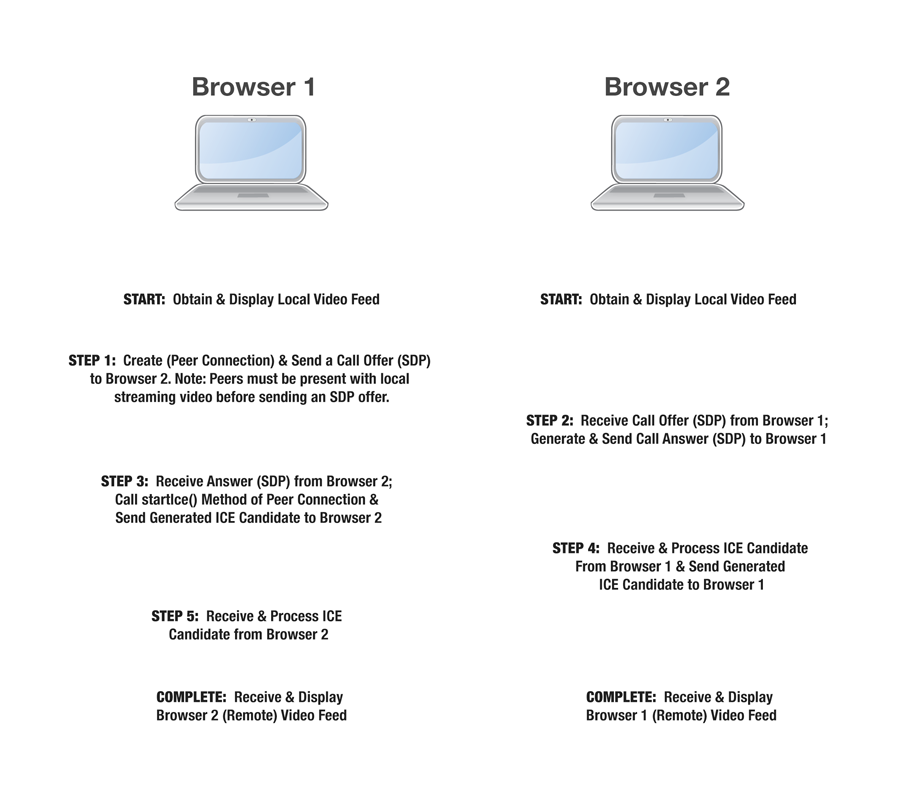
\includegraphics[height=0.50\textheight,natwidth=610,natheight=642]{figs/webrtc_diagram.png}
  	\caption{WebRTC two peer communication process\cite{mdn:p2pwebrtc}}
  	\label{fig:webrtc_diagram}
\end{figure}

\subsection{MediaStream API}

\par The MediaStream \gls{api} represents synchronized streams of media. For example, a stream taken from camera and microphone input has synchronized video and audio tracks. In order to obtain local media, the start step for both peers in Figure \ref{fig:webrtc_diagram} which is a communication process to set up call process from caller peer, the \gls{webrtc} \gls{api}s provide \textit{navigator.getUserMedia()} function to get the video and audio stream from user. For privacy reasons, a web application’s request for access to a user’s microphone or camera will only be granted after the browser has obtained permission from the user. Each MediaStream has an input, which might be a MediaStream generated by \textit{navigator.getUserMedia()}, and an output, which might be passed to a video element or an \textit{RTCPeerConnection}.
\par The \textit{getUserMedia()} method takes three parameters:

\begin{itemize}[topsep=-1em,parsep=0em,itemsep=0em]
 \item A constraints object.
 \item A success callback which, if called, is passed a MediaStream.
 \item A failure callback which, if called, is passed an error object.
\end{itemize}

\par The Code Snippet \ref{code:get_user_media} shows that how the prototype application implements \textit{getUserMedia()} function, it is encapsulated in \textit{WebRTCService} (service is a reusable business logic independent of views in prototype application regarding to AngularJs framework\footnote{AngularJS is an open-source web application framework, maintained by Google and community, that assists with creating single-page applications, one-page web applications that only require HTML, CSS, and JavaScript on the client side.\cite{wiki:angularjs}}). There will be more discuss about prototype application framework in the later part of this chapter. For the constraints object in parameters, the prototype application set 'audio' and 'video' value to true because it is necessary for the real-time communication application to have video and audio stream both.

\begin{lstlisting}[caption={Get User Media Stream function},label={code:get_user_media}]
var media_constraints = {audio: true,video: true};

function _setMediaStream(){
	WebRTCService.getUserMedia(media_constraints,
  								_handleUserMedia,
  								_handleUserMediaError);
  	console.log('Getting user media with constraints', 
  				media_constraints);
}
\end{lstlisting}

\par \textit{getUserMedia()} function is currently available in Chrome, Opera and Firefox. Almost all of the \gls{webrtc} \gls{api}s are slightly different based on different browsers implementation. In the Code Snippet \ref{code:webrtc_service}, from line 40 to line 103 is to make all the set up process for FireFox and from line 106 to line 175 is to make the same set up process for Google Chrome. Because \gls{webrtc} is not standard Web \gls{api} yet, so the implementation on different browsers are different and the \gls{webrtc} \gls{api}s names are slightly different in some browsers. For example, in the Code Snippet \ref{code:webrtc_service} showing, the \textit{RTCPeerConnection} \gls{api} in Firefox is \textit{mozRTCPeerConnection} but in Google Chrome it is \textit{webkitRTCPeerConnection}. In order to make the \gls{webrtc} application works on more browsers, the client side need to figure out which kind of browser is using on the machine then call the corresponding \gls{webrtc} \gls{api}s. Google provides a JavaScript shim called \textit{adapter.js}. It is maintained by Google, it abstracts away browser differences and spec changes. For Angularjs framework used by prototype application, then the \textit{WebRTCService} is implemented to be integrated with \textit{adapter.js} function to achieve the goal of compatibility.

\par However, the prototype application in this thesis will only focus on Google Chrome browser\footnote{Google Chrome is a freeware web browser developed by Google. It used the WebKit layout engine until version 27 and, with the exception of its iOS releases, from version 28 and beyond uses the WebKit fork Blink.\cite{wiki:google_chrome}} to simplify the development process because \gls{webrtc} lower level implementation on different browser s are different and hard to track the issues. Then most of the results in this thesis is based on the application performance of Google Chrome browser. The reason to choose Google Chrome browser rather than other browser because \gls{webrtc} is the technology rapidly pushed by Google and Google Chrome browser has the most market share in the world. As of March 2014, StatCounter estimates that Google Chrome has a 43\% worldwide usage share of web browsers, making it the most widely used web browser in the world.\cite{wiki:google_chrome} However, Google changes a lot to improve the performance of \gls{webrtc} on Google Chrome browser, then it makes the \gls{webrtc} \gls{api}s work different on different version of Google Chrome browser. In the Code Snippet \ref{code:webrtc_service}, from line 124 to line line 136 is the sample case to distinguish the difference among different version of Google Chrome to handle the \textit{RTCPeerConnection} \gls{ice} server constraint implementation.

\par Since \gls{webrtc} \gls{api}s is not standard \gls{api} yet, the prototype application in this thesis will not pay too much work-load on compatibility for different browsers platform. More detail about this issue will be discussed in the Chapter \ref{chp:future_work}.

\subsection{RTCPeerConnection API}

\noindent To set up peer connection, the \textit{RTCPeerConnection} \gls{api} sets up a connection between two peers. In this context, “peers” means two communication endpoints on the World Wide Web. Instead of requiring communication through a server, the communication is direct between the two entities. In the specific case of \gls{webrtc}, a peer connection is a direct media connection between two web browsers. This is particularly relevant when a multi-way communication such as a conference call is set up among three or more browsers. Each pair of browsers will require a single peer connection to join them, allowing for audio and video media to flow directly between the two peers. 

\par To establish peer connection, it requires a new \textit{RTCPeerConnection} object. The only input to the \textit{RTCPeerConnection} constructor method is a configuration object containing the information that \gls{ice}, will use to “punch holes” through intervening \gls{nat} devices and firewalls. The Code Snippet \ref{code:create_peer_connection} shows the create \textit{RTCPeerConnection} object and set three listener (\textit{onicecandidate},\textit{onaddstream},\textit{onremovestream}) to trigger the handlers to deal with the \gls{ice} candidate event and remote stream add/remove events.

\par The \textit{RTCPeerConnection} \gls{api} has two arguments to set, one is configuration object for peer connection and the other is constraint object (set transparent protocol and encryption) for peer connection, these value are shown in Code Snippet \ref{code:create_peer_connection} line 1 to line 10. In the showing case, the prototype is using \gls{stun} servers for different browser aspect, and set the \gls{rtc} channel encryption protocol to \gls{dtls}\footnote{In information technology, the Datagram Transport Layer Security (DTLS) protocol provides communications privacy for datagram protocols. DTLS allows datagram-based applications to communicate in a way that is designed to prevent eavesdropping, tampering, or message forgery.\cite{wiki:dtls}} and enable the \gls{rtc} DataChannel.

\par Because in Firefox, \gls{webrtc} media transparent channel is only based on \gls{dtls} protocol, and in latest version Google Chrome, it is support, then in the prototype application, it will use \gls{dtls} protocol to exchange the media stream.

\par There are two \gls{api}s to handle the \textit{IceCandidate} object which contains \gls{ice} information data. One is \textit{onicecandidate} listener to trigger the function to handle the new \textit{IceCandidate} data object. The other one is \textit{addIceCandidate} function, which is shown in the Code Snippet \ref{code:add_remote_ice}, to add the new \textit{IceCandidate} data object to the remote/local peer connection session description field. 

\begin{lstlisting}[caption={Create Peer Connection function},label={code:create_peer_connection}]
pc_config = WebRTCService.webrtcDetectedBrowser() === 'firefox' ?
  			{'iceServers':[{'urls':'stun:stun.services.mozilla.com'}]} :
  			{'iceServers':[{'urls': 'stun:stun.l.google.com:19302'}]};

pc_constraints = {
			  'optional': [
			    {'DtlsSrtpKeyAgreement': true},
			    {'RtpDataChannels': true}
			  ]
			};
			
function _createPeerConnection(){

	try {
		pc = WebRTCService.peerConnection(pc_config, pc_constraints);
		pc.onicecandidate = _handleIceCandidate;
		console.log('Created RTCPeerConnnection with:\n' +
		      '  config: \'' + JSON.stringify(pc_config) + '\';\n' +
		      '  constraints: \'' + JSON.stringify(pc_constraints) + '\'.');
	} catch (e) {
		console.log('Failed to create PeerConnection, exception: ' + e.message);
		alert('Cannot create RTCPeerConnection object.');
		return;
	}
	pc.onaddstream = _handleRemoteStreamAdded;
	pc.onremovestream = _handleRemoteStreamRemoved;

}
\end{lstlisting}

\begin{lstlisting}[caption={Add Remote IceCandidate function},label={code:add_remote_ice}]
var candidate = WebRTCService.RTCIceCandidate({
					    	sdpMLineIndex:data.content.label,
					    	sdpMid:data.content.id,
					    candidate:data.content.candidate
				});
pc.addIceCandidate(candidate);

\end{lstlisting}

\par In the step 2 of Figure \ref{fig:webrtc_diagram}, after the caller \textit{RTCPeerConnection} run \textit{createOffer()} function to send offer to callee through signaling channel, the callee need run \textit{createAnswer()} function to ask the \gls{stun}/\gls{turn} server to find the path for each other peer and create the answer with \gls{sdp} content. \gls{sdp} is intended for describing multimedia communication sessions for the purposes of session announcement, session invitation, and parameter negotiation. \gls{sdp} does not deliver media itself but is used for negotiation between end points of media type, format, and all associated properties.\cite{wiki:sdp} Before \textit{RTCPeerConnection} use \textit{createOffer()} function to send a \gls{webrtc} offer to the callee, it is required to be present with local streaming video, like Figure \ref{fig:webrtc_diagram} mentioned.

\par The sample \gls{sdp} from the prototype application is shown in Code Snippet \ref{log:webrtc_answer_sdp}. Line 2 in Code Snippet \ref{log:webrtc_answer_sdp} is the field 'o', it describes originator, session identifier, username, id, version number and network address. It usually means that where this package comes from. Line 7 and line 17 are field 'm', it describes media name and transport address. And line 11,12 and line 27,28 are the relevant lines for audio and video media field, they describes media filed 'candidate' attributes, in the sample case of Code Snippet \ref{log:webrtc_answer_sdp}, they are the \gls{ice} candidate from the \gls{stun}/\gls{turn} server. These are important fields regarding to the prototype system because they are used in XMS server and application server of the prototype system.

\begin{lstlisting}[caption={Sample \gls{webrtc} Answer \gls{sdp}},label={log:webrtc_answer_sdp}]
sdp: v=0
o=xmserver 1399363527 1399363528 IN IP4 10.254.9.135
s=xmserver
c=IN IP4 10.254.9.135
t=0 0
a=ice-lite
m=audio 49152 RTP/SAVPF 0 126
a=rtpmap:0 PCMU/8000
a=sendrecv
a=rtcp:49153
a=candidate:1 1 UDP 2130706431 10.254.9.135 49152 typ host
a=candidate:1 2 UDP 2130706430 10.254.9.135 49153 typ host
...
a=acfg:1 t=1
a=rtpmap:126 telephone-event/8000
a=fmtp:126 0-15
m=video 57344 RTP/SAVPF 100
b=AS:1000
a=rtpmap:100 VP8/90000
a=fmtp:100 max-fr=30; max-fs=1200
a=sendrecv
a=rtcp:57345
a=rtcp-fb:100 ccm fir
a=rtcp-fb:100 nack
a=rtcp-fb:100 nack pli
a=rtcp-fb:100 goog-remb
a=candidate:2 1 UDP 2130706431 10.254.9.135 57344 typ host
a=candidate:2 2 UDP 2130706430 10.254.9.135 57345 typ host
...
\end{lstlisting}

\par In the step 3 of Figure \ref{fig:webrtc_diagram}, the caller will receive the answer from callee and process it by adding the remote \gls{sdp} to \textit{RTCPeerConnection}, like the Code Snippet \ref{code:add_remote_ice}. By the meantime, the step 4 of Figure \ref{fig:webrtc_diagram}, the callee will receive the \gls{sdp} from caller with the \gls{ice} candidate information data, and process it the same way as caller does, add some to \textit{RTCPeerConnection} object by \textit{addIceCandidate()} function.

\par \gls{webrtc} clients (known as peers) also need to ascertain and exchange local and remote audio and video media information, such as resolution and codec capabilities. Signaling to exchange media configuration information proceeds by exchanging an offer and an answer using the \gls{sdp}. The \textit{createOffer()} function and \textit{createAnswer()} function both have callback function to handle the \gls{sdp} either to call \textit{setLocalDescription()} by caller or call \textit{setRemoteDescription()} by callee when callee gets the caller's \gls{sdp} from \gls{webrtc} offer. The Code Snippet\ref{log:webrtc_answer_sdp} shown is the \gls{webrtc} answer \gls{sdp} from the callee when the callee end-point decide to accept this conversion session.

\par Once the \textit{RTCPeerConnection} is established, the client need configure where the media or data to store and display if it is necessary. In the prototype application of this thesis, media stream will be displayed in a \gls{html5} tag called \textit{<video>}. It will only be shown when there is media stream in \textit{<video>} tag source.

\section{Prototype Implementation Framework}

\noindent Since \gls{webrtc} is a web \gls{api}, the prototype application will be a web application. There are many different web application framework nowadays to provide rich-client web application. In this section, some of the web application framework will be discussed to figure out which framework is best solution to the prototype scenario. Furthermore, application server will be discussed with different implementation solutions since it does signaling and bridge the \gls{sip} network and clients.

\subsection{Client Implementation Framework}

\noindent To choose web application framework to implement the client application in this thesis scenario, the main fact is that if the web  application framework is fit to the real time communication application and if the framework has the ability to integrate with \gls{webrtc} \gls{api}. After research about these kinds of web application framework, it narrows down to three main framework to discuss.

\textbf{AngularDart :}

\par AngularDart is a framework for building web-apps in Dart. Dart is an open-source Web programming language developed by Google. It is a class-based, single inheritance, object-oriented language with C-style syntax. It supports interfaces, abstract classes, reified generics, and optional typing. Static type annotations do not affect the runtime semantics of the code. Instead, the type annotations can provide documentation for tools like static checkers and dynamic run time checks.\cite{wiki:dart} Because most of the script language is not type strict, it is easy to mess up the code and value type in script language. Moreover, Dart has Dart-to-JavaScript compiler,dart2js, it makes Dart can be used in client and server both. Addition to AngularJs framework in Dart, it provide a professional web application structure to the developer to implement. More about AngularJs notable features will be covered in the later AngularJs solutions. 

\par The \gls{webrtc} implementation in Dart is in this repository: \url{https://github.com/br1anchen/AngularDart_webRTC}. The Code Snippet \ref{code:dart_webrtcctrl} shows the main controller in AngularDart. The line 5 is to import \gls{webrtc} client class \textit{speack\_client.dart}, the class has all the \gls{webrtc} \gls{api}s implemented in Dart. Line 23 is to initialize the \textit{SpeakerClient} object and set the arguments WebSocket url and room name. They are used for signaling in WebSocket Protocol.

\par However, after implementation of client application and server back-end in Dart. There is a critical bug in the current Dartium browser. The Dart SDK ships with a version of the Chromium web browser modified to include a Dart \gls{vm}. Dartium browser can run Dart code directly without compilation to JavaScript. It is intended as a development tool for Dart applications, rather than as a general purpose web browser. When embedding Dart code into web apps, the current recommended procedure is to load a bootstrap JavaScript file, "dart.js", which will detect the presence or absence of the Dart \gls{vm} and load the corresponding Dart or compiled JavaScript code, respectively, therefore guaranteeing browser compatibility with or without the custom Dart VM.\cite{wiki:dart} 
\par The issue noticed as \textbf{RtcPeerConnection.addIceCandidate results in a NotSupportedError: Internal Dartium Exception} in the Dart Google Project issues.\cite{bug:dartium} The sample code in the \gls{webrtc} Dart implementation shown in Code Snippet \ref{code:dart_add_ice}, line 1 is to create \textit{RTCPeerConnection} object. From line 5 to line 13 is to send message to server when \textit{RTCPeerConnection} object get \textit{onIceCandidate} event witch \gls{ice} candidate information. Line 17 is to bind the message listener event to Dart function \textit{onCandidate.listen}. From line 21 to line 30 is the Dart function to create \textit{RTCIceCandidate} object and add to \textit{RTCPeerConnection} object. The bug issue happens on line 27, when the \textit{RTCPeerConnection} call \textit{addIceCandidate} function, it is not allowed to have callback function in current version Dartium.

\begin{lstlisting}[caption={Add IceCandidate in Dart},label={code:dart_add_ice}]
var pc = new RtcPeerConnection(_iceServers, _dataConfig);

....

    pc.onIceCandidate.listen((e){
      if (e.candidate != null) {
        _send('candidate', {
          'label': e.candidate.sdpMLineIndex,
          'id': id,
          'candidate': e.candidate.candidate
        });
      }
    });
    
...

get onCandidate => _messages.where((m) => m['type'] == 'candidate');

...

onCandidate.listen((message) {
	var candidate = new RtcIceCandidate({
		'sdpMLineIndex': message['label'],
        'candidate': message['candidate']
    });

    _connections[message['id']].addIceCandidate(candidate,(){},(e){
    		print('add ice candidate error');
    });
});

...
\end{lstlisting}

\par There is a work around solution in one Stack Overflow\footnote{Stack Overflow is a privately held website, the flagship site of the Stack Exchange Network, created in 2008 by Jeff Atwood and Joel Spolsky, as a more open alternative to earlier Q\&A sites such as Experts Exchange.} answer: \url{http://stackoverflow.com/questions/20404312/how-to-call-addicecandidate-in-dart}. The fix method is to use \textit{js-interop} library to use pure JavaScript code in Dart to call the \gls{webrtc} Web \gls{api} instead of Dart \gls{webrtc} interface.
\par Mozilla's Brendan Eich, who developed the JavaScript language, stated that:

\textit{"I guarantee you that Apple and Microsoft (and Opera and Mozilla, but the first two are enough) will never embed the Dart VM. So 'Works best in Chrome' and even 'Works only in Chrome' are new norms promulgated intentionally by Google. We see more of this fragmentation every day. As a user of Chrome and Firefox (and Safari), I find it painful to experience, never mind the political bad taste."}\cite{wiki:dart}

\par Since Dart in not support to most modern web browser like FireFox, will not be used in this prototype.

\textbf{Sipml5 + webrtc2sip:}

\begin{figure}
	\centering
    	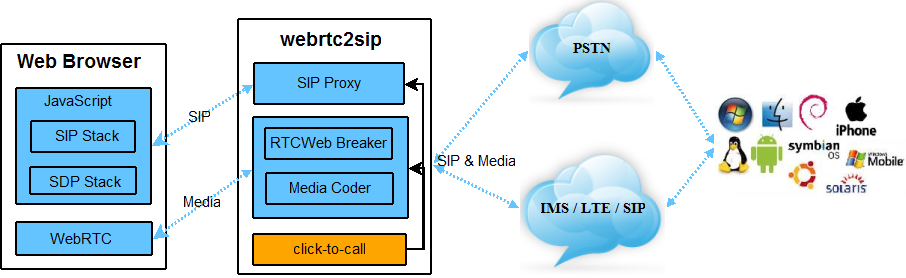
\includegraphics[width=0.80\textwidth,natwidth=610,natheight=642]{figs/sipml5_network.png}
  	\caption{Sipml5 and webrtc2sip Network}
  	\label{fig:sipml5_network}
\end{figure}

\par Sipml5 is the world's first open source \gls{html5} \gls{sip} client entirely written in JavaScript for integration in social networks (FaceBook, Twitter, Google+), online games, e-commerce websites, email signatures. The media stack rely on \gls{webrtc}. The client can be used to connect to any \gls{sip} or \gls{ims} network from your preferred browser to make and receive audio/video calls and instant messages.\cite{website:sipml5}

\par Sipml5 provides whole client solution to communicate with other kind of signaling real-time communication network. The \gls{sip} and \gls{sdp} stacks are entirely written in JavaScript and the network transport uses WebSockets as per draft-ibc-sipcore-sip-websocket. However the community of sipml5 is not so active, the issues and source code on sipml5 source code project website \url{https://code.google.com/p/sipml5/} are not updated regularly. Like the Figure \ref{fig:sipml5_network} showing, it works with media gateway webrtc2sip.

\par webrtc2sip is a smart and powerful gateway using \gls{webrtc} and \gls{sip} to turn your browser into a phone with audio, video and \gls{sms} capabilities. The gateway allows your web browser to make and receive calls from/to any \gls{sip}-legacy network or \gls{pstn}.
The gateway contains four modules: \gls{sip} Proxy, RTCWeb Breaker, Media Coder, Click-to-Call.\cite{website:webrtc2sip}

\par In the prototype working scenario, it is necessary to have media gateway to communicate with \gls{sip}-legacy network. Since the current \gls{pstn} using in this prototype go through Gintel \gls{mpbx} Platform, it is necessary to use RTCWeb Breaker to be able to connect the browser to a SIP-legacy endpoint.

\par Therefore, the test for Sipml5 and webrtc2sip solution is based on the live demo \url{http://sipml5.org/call.htm}. But even with the RTCWeb Breaker, the test is still failed to call any number through the target \gls{pstn}. Since most of the source code of these two framework are hidden from the encapsulation, it is impossible to debug which part of the testing system is the problem. In the test, the registration for \gls{sip} client is successful, but there are 'too long message' in the \gls{sip} error message got from the \gls{sip} server. It means that the sipml5 and webrtc2sip network architecture is not compatible with the target \gls{pstn} through the Gintel \gls{mpbx} Platform. This solution can not be used in the prototype system.

\textbf{AngularJs + Socket.IO:}

\par AngularJS is built around the belief that declarative programming should be used for building user interfaces and wiring software components, while imperative programming is excellent for expressing business logic. The framework adapts and extends traditional \gls{html} to better serve dynamic content through two-way data-binding that allows for the automatic synchronization of models and views. As a result, AngularJS de-emphasizes \gls{dom} manipulation and improves testability. Angular follows the \gls{mvc} pattern of software engineering and encourages loose coupling between presentation, data, and logic components. Using dependency injection, Angular brings traditional server-side services, such as view-dependent controllers, to client-side web applications. Consequently, much of the burden on the backend is reduced, leading to much lighter web applications.\cite{wiki:angularjs}

\par AngularJs is perfect for single-page web application, the framework features provide developer a professional way to structure the web application in JavaScript. Moreover, the developer community of AngularJs is quite active, there are a lot of different Angular module services to provide the different interfaces against different web \gls{api}s.In the prototype, there will be several third party Angular module library to be used in order to integrate with some advanced JavaScript library or web \gls{api}s in Angular style.

\par Socket.IO is a JavaScript library for realtime web applications. It has two parts: a client-side library that runs in the browser, and a server-side library for node.js. Both components have a nearly identical \gls{api}. Socket.IO primarily uses the WebSocket protocol, but if needed can fallback on multiple other methods, such as Adobe Flash sockets, \gls{jsonp} polling, and \gls{ajax} long polling, while providing the same interface. Although it can be used as simply a wrapper for WebSocket, it provides many more features, including broadcasting to multiple sockets, storing data associated with each client, and asynchronous I/O.\cite{wiki:socketio} In the prototype application, Socket.IO is used in WebSocket protocol because the WebSocket protocol provides full-duplex communications channels over a single \gls{tcp} connection. Then the communication channel will be active and real time between the clients and server during the whole connecting procedure. It fits the real time communication application requirement.

\par After test demo client application implemented in AngularJs and Socket.IO frameworks, it works fine with the basic \gls{webrtc} functions and simple \gls{sip} registration against \gls{sip} server to target \gls{pstn}. The final decision of the client implementation framework of prototype system will be AngularJs and Socket.IO.

\subsection{Server Implementation Framework}

\noindent Since the client side will use Socket.IO as communication protocol library, the server back-end in the prototype system will use Node.js as server implementation framework. In thist section, more detail about comparison and differences of Node.js against traditional web service back-end (in Java, ASP .NET or \gls{php}) will be covered.

\textbf{Node.js:}

\par 

\textbf{Mobicents Sip Servlets + Java web service:}

\par 